\documentclass[a4paper,12pt]{article}
\usepackage{comment}
\usepackage{import}
%citepath="/home/bruno/users/weh40/sims_phosim/data/SEDs/SEDs" # my default path
%dirlist=["BD_H2O_1", "BD_O3_1run", "BD_O2_1run", "H2O-new_4run-img", "H2O-aperture_1run", "O3_2run-100", "O2_1run" ]


\usepackage{xspace} 
\usepackage{graphicx}
\usepackage{subfig}
\usepackage{float}
\usepackage{placeins}
\usepackage[document]{ragged2e}

\DeclareGraphicsExtensions{.pdf,.png}
\graphicspath{{/home/bruno/users/weh40/Pictures/}}
\newcommand{\citp}{/home/bruno/users/weh40/sims_phosim/data/SEDs/SEDs/back/}
\newcommand{\fa}{BD_H2O_1/}
\newcommand{\fb}{BD_O3_1run/}
\newcommand{\fc}{BD_O2_1run/}
\newcommand{\fd}{H2O-new_4run-img/}
\newcommand{\fe}{H2O-aperture_1run/}
\newcommand{\ff}{O3_2run-100/}
\newcommand{\fg}{O2_1run/}
\let\oldtabular\tabular
\renewcommand{\tabular}{\footnotesize\oldtabular}
\usepackage{amsmath}
\begin{document}

\title{Report on numerical simulation of photometry variation with water vapor}
\author{Wei Hu}
\maketitle

\justify

Water vapor in the Earth's atmosphere creates a significant and variable source of absorption in photometry of astronomical sources.  This is particularly acute in the y (and z) optical bands.
\paragraph{}

We here demonstrate the feasibility of determining the precipitable water vapor during an exposure by observing the shifts in y- (and z-band) magnitudes as a function of colors like g-r, g-z, g-y.




\clearpage
\tableofcontents
\clearpage

\section{Scope and Goals}


Methods: We simulate observations of 526 white drawf and 4886 main sequence stars in the LSST PhoSim SED library and propagate through nominal filters and system throughput produced via ModTran .  This simulation is done purely through numeric integration of the SEDs, instrument throughput, and atmospheric transmission, the result of which can be compared and verified by Photon Simulator (Phosim) \cite{manual}.
\paragraph{}
We use a grid of atmospheric parameters to generate a suite of simulated observations.  We then fit for the value of the H2O column density using a fitting function (of no more than 19 parameters) that uses, e.g., the observed bands magnitudes g, r, z, y, as compared to the true bands magnitudes g, r, z, y; and g-r, g-z, g-y colors,  to predict the H2O column density.

\graphicspath{{/home/bruno/users/weh40/sims_phosim/data/SEDs/SEDs/back/4thrun/}}
\begin{figure}[h!]
\begin{center}
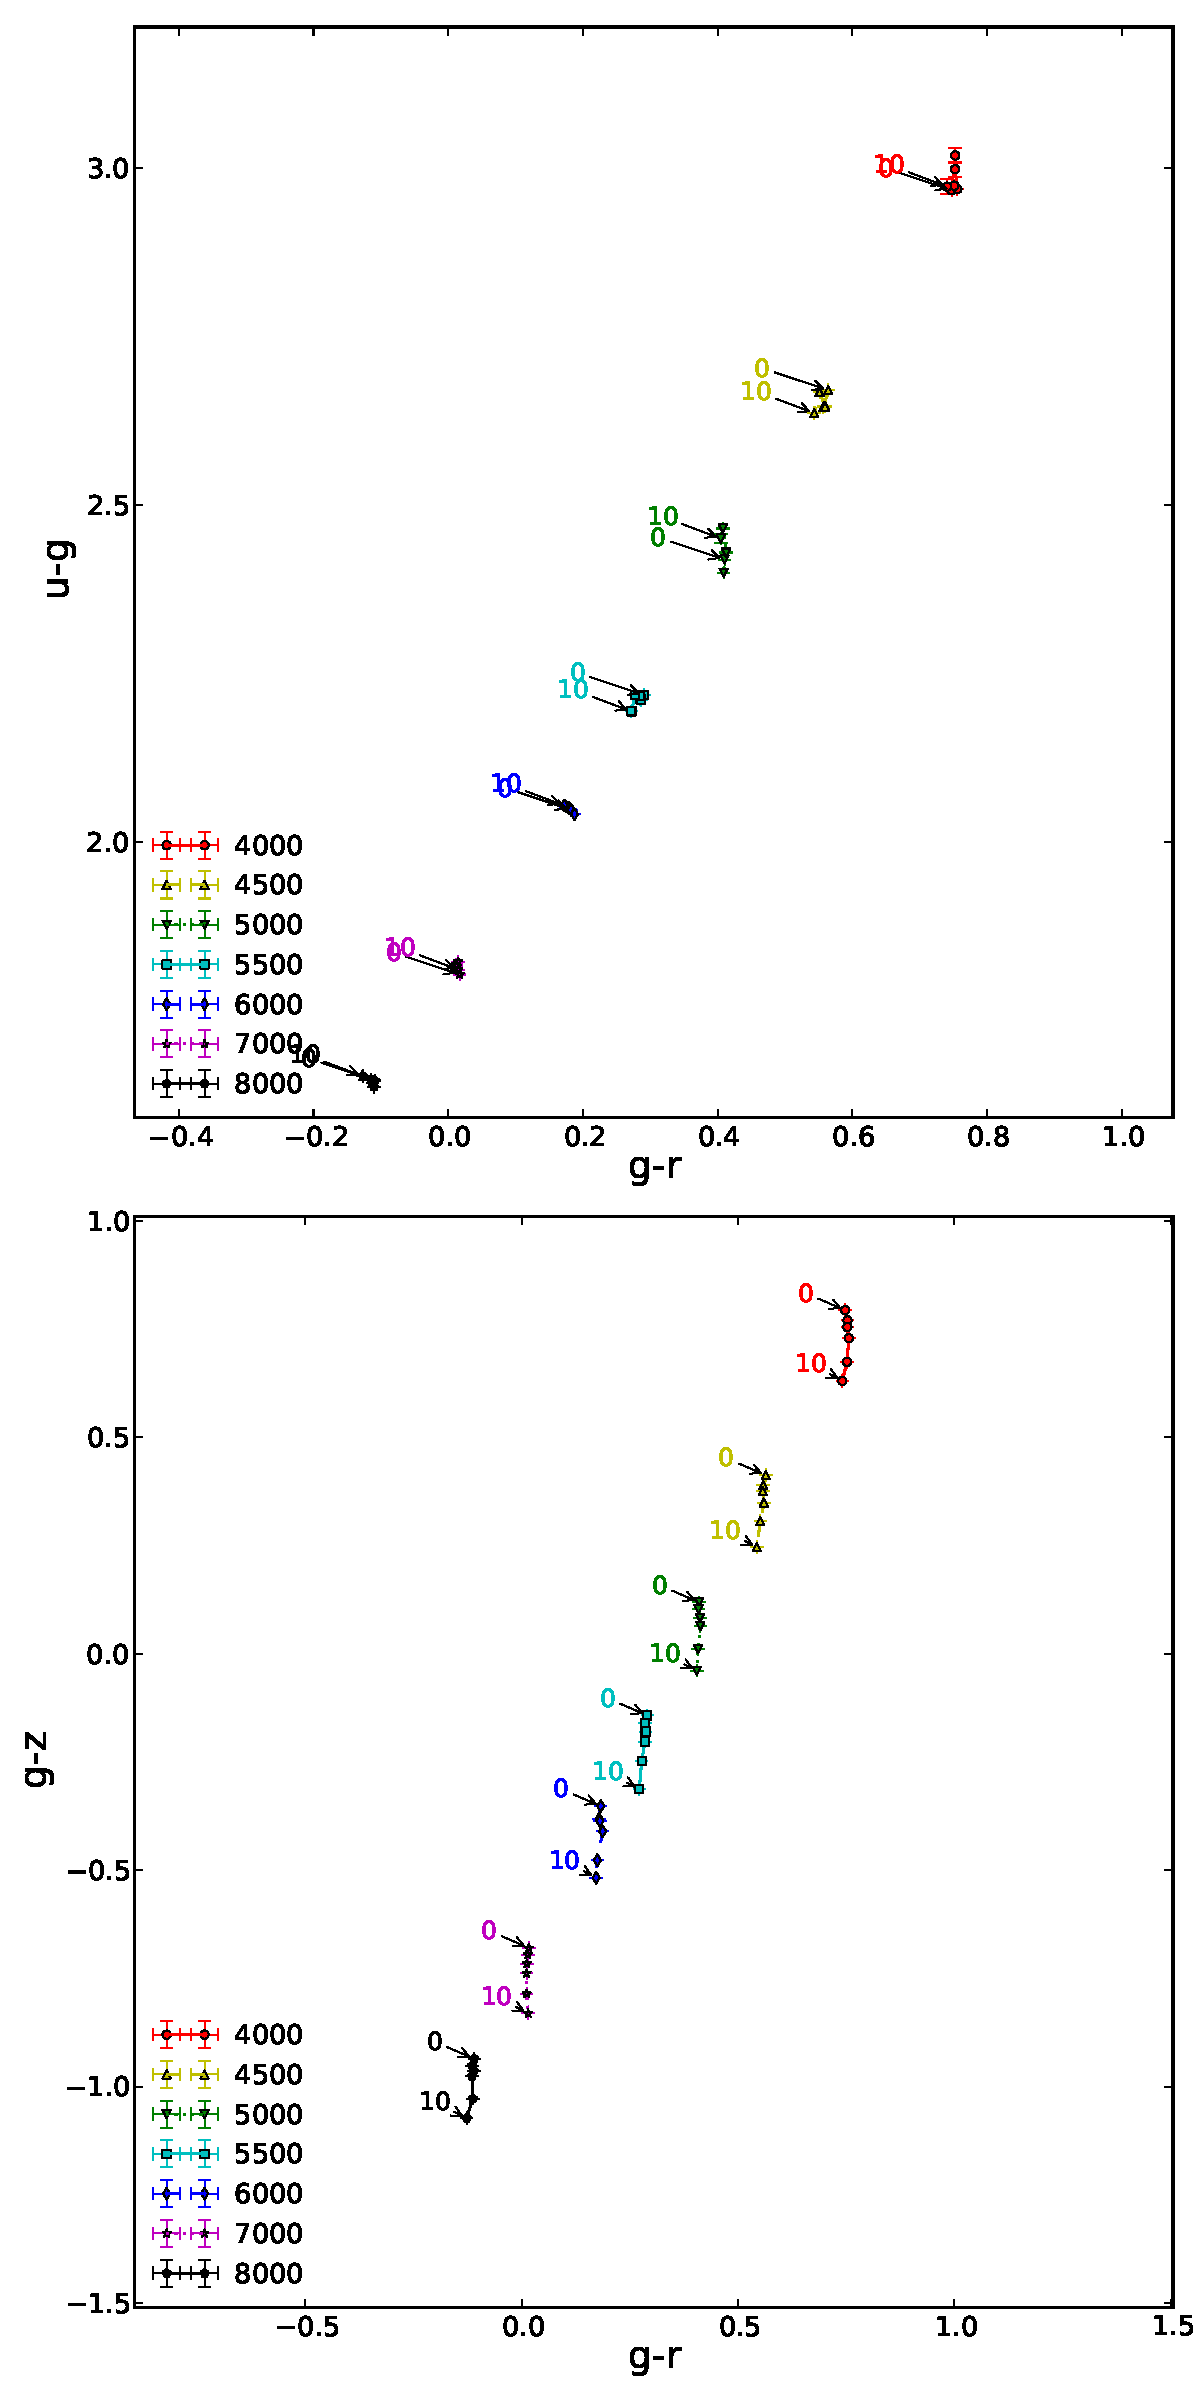
\includegraphics[page=1,width=0.7\textwidth,trim=1mm 1.5mm 1mm 205mm,clip=true,angle=0]{color-color}
\caption{color\_color diagram for Black Body spectra, with variation vs LSST norm value indicated (0-10, corresponding to 0 - 138.6 mm of PWV), norm is easy to label here.}
\end{center}
\end{figure}


\paragraph{}
\paragraph{}


The expected senario is that an extensive 2D (or multidimensional) color\_color diagram is filled with SEDs which have relatively smooth spectra and continuous trend along HR diagram. As a result, an analytic model can be deduced, such that we can get a convenient vector fields of correction dependent on specific locus on the color\_color plane (or hyperplane). 

However, in practice a number of issues come into play, like the peculiarities of SEDs from certain source, which may not have a continuous and smooth trend along color-axes on the diagam.



\subsection{Background: LSST Parameters}

Our numerical simulation is based on comparison with the Phosim result. We list the conversion of Phosim parameters to real units, as well as range of variation of gases in reality, including $H_{2}O$, $O_{3}$, and $O_{3}$. The column densities and LSST norm values are obtained by vertical integration of the relevant profiles in the phosim database.

\rm{$H_2O$}: LSST defalut column density (ie. norm): (Column integration of h2oprofile.txt) timing nprofile.txt (vertical profile) 4.633$\times10^{22}/cm^2$ or 13.86 mm in Precipitable water volumn (PWV), 

\rm{- usual variation over a year: 20 times in range or 0.3 - 6 cm in PWV}

\rm{$O_3$}: LSST norm: (Integration of profiles o3profile.txt) 6.838$\times10^{18}/cm^2$=254 Dobson Unit (DU),

\rm{- usual variation over a year: 20-50\%}

\rm{$O_2$}: LSST norm: (Integration of nprofile.txt timing $O_2$ mixing ratio) 4.517$\times10^{24}/cm^2$

\rm{- usual variation over a year: 0.02\%} \cite{atmoswater}

The range of simulation is chosen according to reality.

\section{Input Data}
\subsection{Gases Transmission}

The transmission of gases is calculated using the Beer's law, which has been compared with the phosim results to a range far exceeding the reality (to 100 LSST norm). The difference between the two approaches is small except for the absolute intensities. All the behaviors and patten of residuals are the same, which has been tested by model fit.

The Beer's law:
\begin{equation}
T_{\rm gas}(\lambda)=e^{-\int\sigma(\lambda)N(z)}
\end{equation}
where $\sigma(\lambda)$: cross section
N(z): vertical profiles

In light of this simple relationship, we can calculate gases transmission from cross sections of gases that are used by phosim, after column integration has been done. Below we list examples of water, ozone and oxygen, with column densities or usual values indicated.


\graphicspath{{/home/bruno/users/weh40/Pictures/}}
\clearpage
\centering
Water
\begin{figure}[hb!]
\centering
\subfloat[H$_2$O=3.5 mm\label{subfig_1}]{
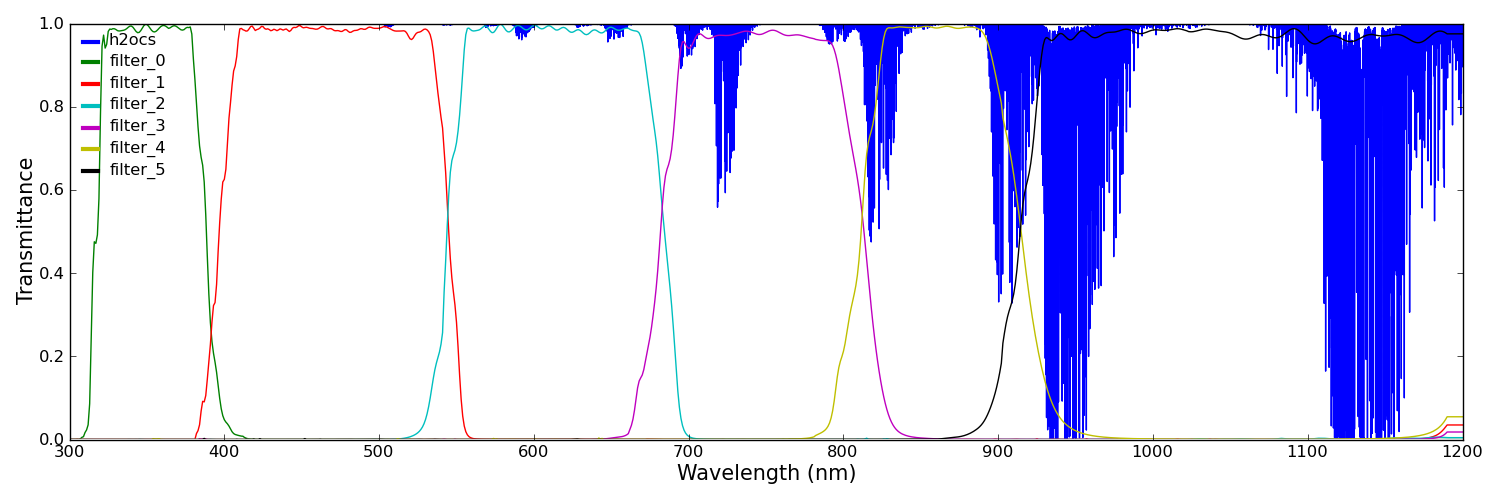
\includegraphics[width=\textwidth,trim=1mm 2mm 1mm 2mm,clip=true,angle=0]{h2ocs-h2ocs_0_1}
}
\subfloat[H$_2$O=14 mm\label{subfig_2}]{
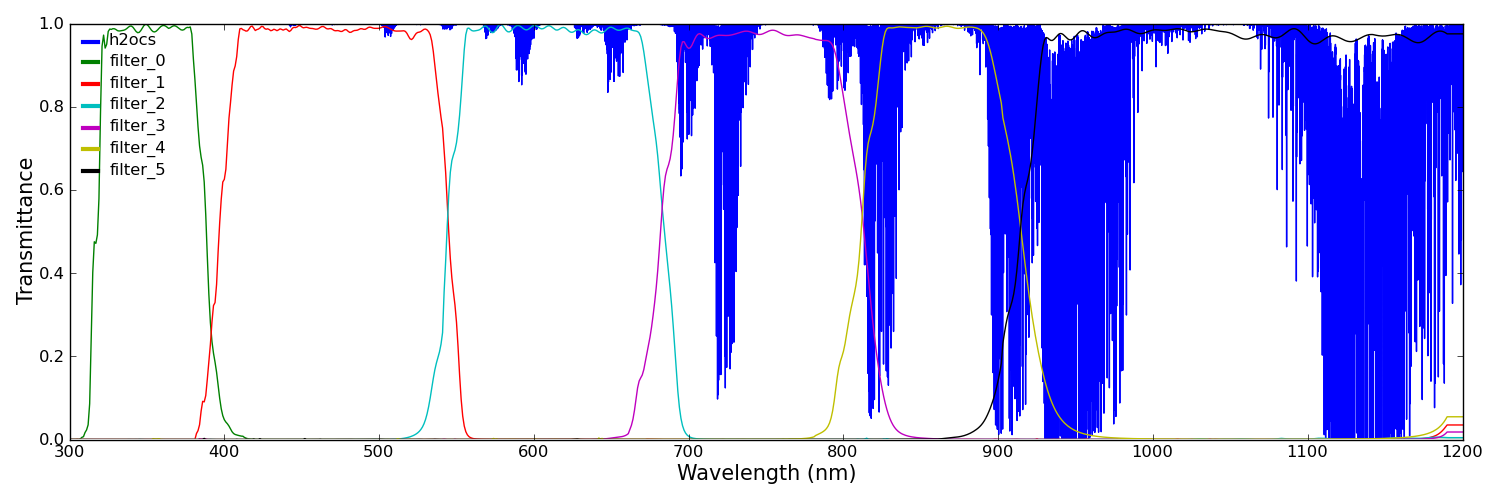
\includegraphics[width=\textwidth,trim=1mm 2mm 1mm 2mm,clip=true,angle=0]{h2ocs-h2ocs_0_4}
}


\caption{H$_2$O transmittance}
\end{figure}

\clearpage
Ozone
\begin{figure}[hb!]
\centering
\subfloat[O$_3$=254 DU\label{subfig_1}]{
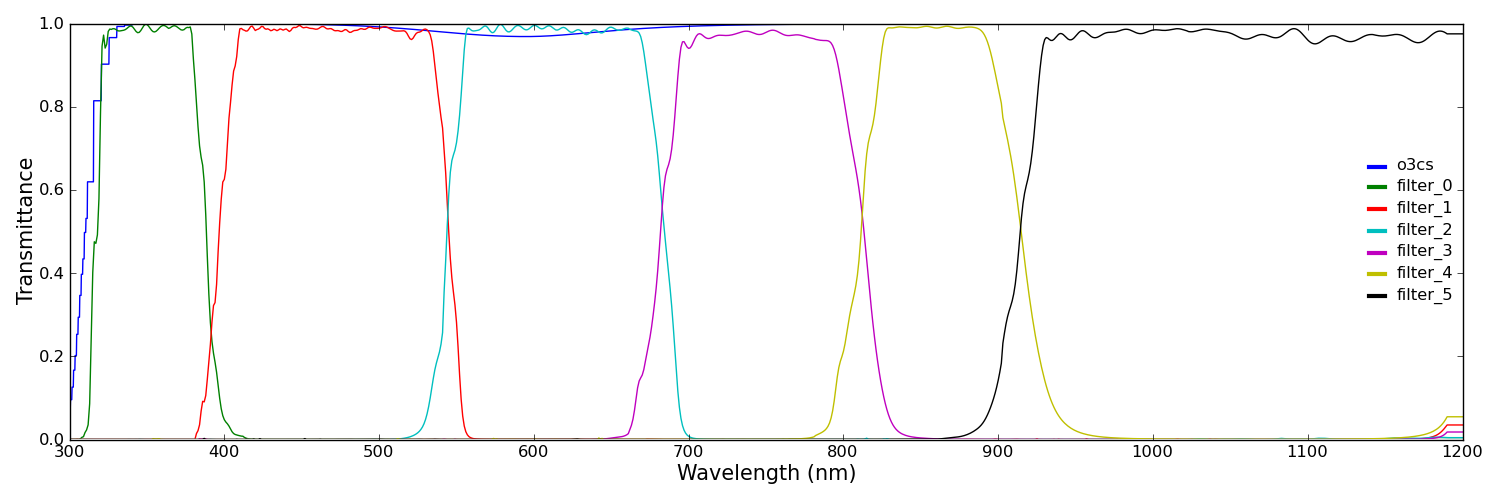
\includegraphics[width=\textwidth,trim=1mm 2mm 1mm 2mm,clip=true,angle=0]{o3cs-o3cs}
}

\caption{O$_3$ transmittance}
\end{figure}

Oxygen
\begin{figure}[hb!]
\centering
\subfloat[O$_2$ for 1 atm air\label{subfig_1}]{
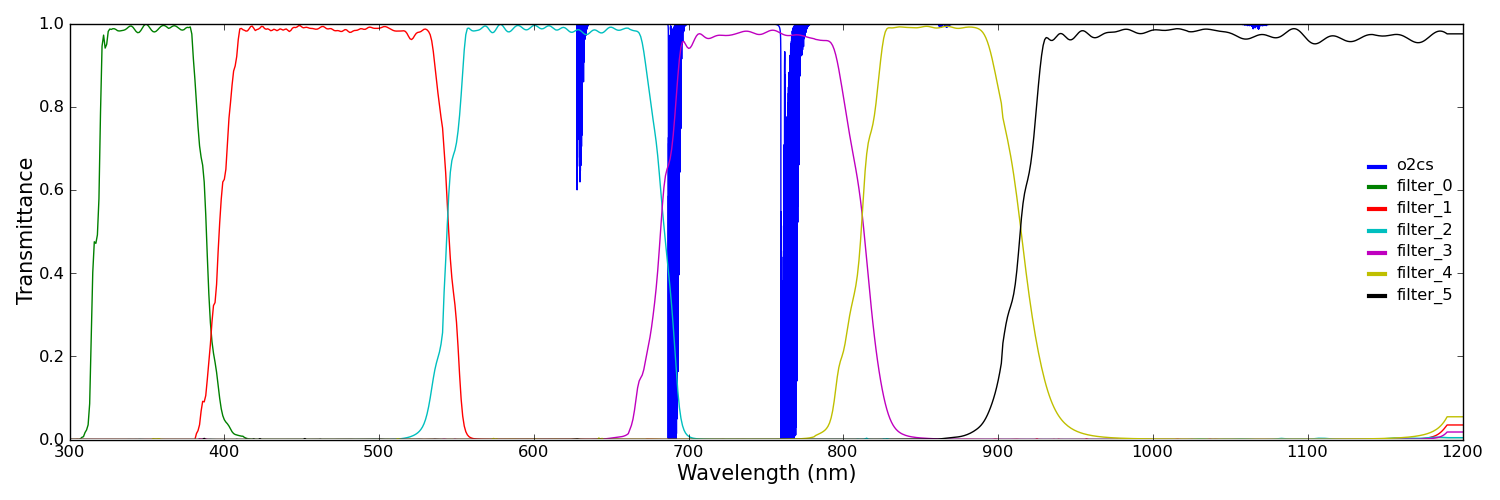
\includegraphics[width=\textwidth,trim=1mm 2mm 1mm 2mm,clip=true,angle=0]{o2cs-o2cs}
}

\caption{O$_2$ transmittance}
\end{figure}

\raggedright
Note that for water, the transmission of 0.4 norm corresponds to that of phosim with 1 norm, so in practice a 'tuning factor' of 0.4 is applied in the integration. In case of ozone and oxgen, tunning factors are not used, for good consistencies with phosim results.

With the help of those transmittances easily obtained, we can see which band would be impacted and how.
 
 \clearpage
\subsection{Database}

The source of data is sims\_sed\_library, a standard LSST SEDs library on which our numerical atmospheric simulation is run. It is available at:

git clone git://dev.lsstcorp.org/LSST/sims/sims\_sed\_library.git

The wDs and kurucz SEDs spectra are found in the folder: 
 sims\_sed\_library/upstream/SEDs/starSED/wDs and 
sims\_sed\_library/upstream/SEDs/starSED/kurucz

,respectively.

\clearpage
\subsection{LSST Throughput}
The figure shows the system throghput calculated by ModTran, combining the Rayleigh scattering, trace gases transmission (CO2, NH3, etc.), the optics (lens, mirrors), the CCD detector, and the filters. The nominal filter responsive curves are drawn in the background for comparison. 
\FloatBarrier
\graphicspath{{/home/bruno/users/weh40/Pictures/5figs/}}
\begin{figure}[h!]
\begin{center}
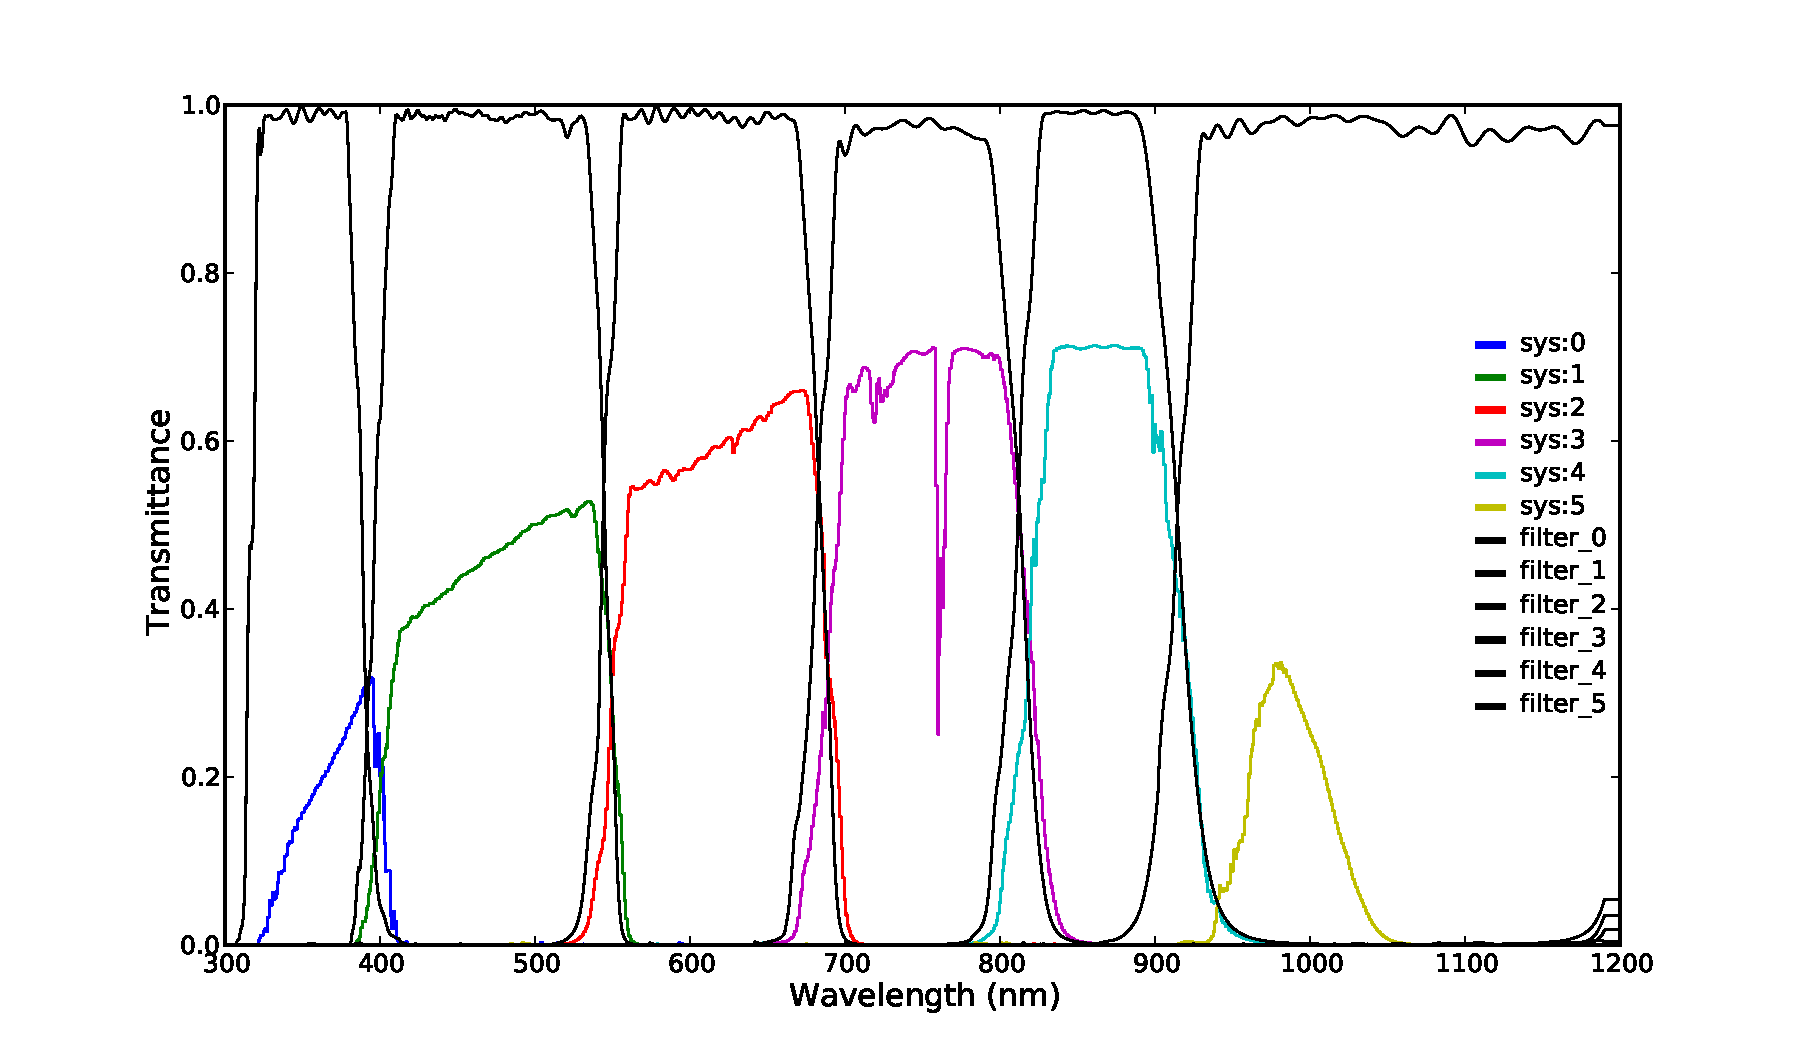
\includegraphics[width=1.2\textwidth,trim=0mm 0mm 0mm 0mm,clip=true,angle=0]{Fig2_sys}
\caption{LSST - Throughput}
\end{center}
\end{figure}
\FloatBarrier



\clearpage
\begin{comment}
\documentclass[a4paper,12pt]{article}
\usepackage{comment}
\usepackage{import}
%citepath="/home/bruno/users/weh40/sims_phosim/data/SEDs/SEDs" # my default path
%dirlist=["BD_H2O_1", "BD_O3_1run", "BD_O2_1run", "H2O-new_4run-img", "H2O-aperture_1run", "O3_2run-100", "O2_1run" ]


\usepackage{xspace} 
\usepackage{graphicx}
\usepackage{subfig}
\usepackage{float}
\usepackage{placeins}
\usepackage[document]{ragged2e}
\usepackage{amsmath}
\usepackage{mathtools}

\DeclareGraphicsExtensions{.pdf,.png}
\graphicspath{{/home/bruno/users/weh40/Pictures/}}
\newcommand{\citp}{/home/bruno/users/weh40/sims_phosim/data/SEDs/SEDs/back/}
\newcommand{\fa}{BD_H2O_1/}
\newcommand{\fb}{BD_O3_1run/}
\newcommand{\fc}{BD_O2_1run/}
\newcommand{\fd}{H2O-new_4run-img/}
\newcommand{\fe}{H2O-aperture_1run/}
\newcommand{\ff}{O3_2run-100/}
\newcommand{\fg}{O2_1run/}
\newcommand{\R0}{Intcolors/tpxall_R0_order0/}
\let\oldtabular\tabular
\renewcommand{\tabular}{\footnotesize\oldtabular}
\usepackage{amsmath}
\begin{document}
\end{comment}


\section{Results}

\subsection{wDs}


With scipy.optimize.minimize, multiple dimensional fit can be done relatively fast and easily.

In practice, we will choose a power function, which leads to slightly improved error compared with the logarithmic function. 

Specifically, we prefer $y_{\rm power} = (bx_{\rm H2O}+1)^I -1$ over $y_{\rm log} = log_{10}(bx_{\rm H2O}+1)$ from experience. The power function here means the base contains the variable $x_{\rm H2O}$. (the $H_2O$ norm value, as defined in Sec. 1.1), y is the band magnitude shift, b and I are coefficients.

Because of the interdependence of multiple color terms, an approach is to perform a Principal Componnets Analysis (PCA), so as to seperate out the independent dimensions with the most variance. The package for pca is matplotlib.mlab.mlabPCA, which automatically normalizes the variance of each input dimension. In practice, we assumed that dimensions with much less variances in colors can be neglected.

Of 8 colors: u-g, g-r, g-i, g-z, g-y, r-i, r-z, r-y, the intrinsic variances are of order 1: [0.443, 0.337, 0.537, 0.661, 0.790, 0.200, 0.324, 0.454]

The weight coefficients (descaled from the output weight matrix) for first three eigenvectors  are:


W1: [-0.7965731 , -0.79756769, -0.7977423 , -0.79782595, -0.79783285, -0.79773173, -0.7977184 , -0.79736486] ,


W2: [ 2.50661256,  0.49760719,  0.01441818, -0.15567855, -0.31273392,  -0.79864561, -0.83446674, -0.9137465 ],


W3: [  0.6371916 , -0.98133088, -0.69430005, -0.38027843,  0.24019528,  -0.21105062,  0.2444841 ,  1.14636762] 



The fractions of variance for all principal components are:

[  9.99188643e-01,   5.22457527e-04,   2.84454714e-04,   4.18757463e-06,   2.57440701e-07,   3.72234266e-31,   6.94589339e-32,   6.91337479e-33]
Of the first three dimensions, we keep only the first and third one, although the variance of the second dimension is more than twice than that of the third. In fact, we found no appreciable dependence of the fit function on the second dimension (the derivative is ~ 0).

Assuming linearity in colors, the model is:
\begin{subequations}
\begin{equation}
y_{\rm nonlin2}=(b x_{\rm H2O}+1)^{I}-1 - s x_{\rm H2O} +a_{17}x_{\rm H2O}^2+a_{18}x_{\rm H2O}^3  
\end{equation}
\begin{equation}
b = a_0+a_1Y_0+a_2Y_2+a_3x_{\rm O3}+a_4x_{\rm tau}+a_5x_{\rm index}  
\end{equation}
\begin{equation}
I=a_6+a_7Y_0+a_8Y_2+a_9x_{\rm O3}+a_{\rm 10}x_{\rm tau}+a_{\rm 11}x_{\rm index}  
\end{equation}
\begin{equation}
s=a_{\rm 12} + a_{\rm 13}Y_0 + a_{\rm 14}x_{\rm O3} +  a{\rm 15}x_{\rm tau} + a_{\rm 16}x_{\rm index}
\end{equation}
\end{subequations}
where $Y_0$: the first PCA component of colors, $Y_2$: the third PCA component; $x_{\rm H2O}$: the $H_2O$ gas norm, $x_{\rm O3}$: the $O_3$ gas norm. The 'norm' unit is the default value of gas components used in Phosim, can be considered as a typical value, as mentioned before.
$x_{\rm tau}$ and $x_{\rm index}$: the coefficients aerotau and aeroindex in the aerosol optical depth formula: $AOD= aerotau(\frac{\lambda}{0.5\mu m})^{aeroindex}$

\paragraph{}
Of the 1333 wDs stars in the library, we focused on 526 stars selected from : 173 Bergeron 4750-6600K (indices: 177-350) and 352 Bergeron He 6600-30000 
(indices: 980-1332)
\paragraph{}
As a result, the coefficients for the y band are:

a = [5.77154789e+00,  -3.20399873e-02,   1.08998053e+00,   1.55738561e-03,   2.33856994e-01,   4.62531644e-03,  2.00091306e-02,   

2.10643367e-04,  -3.73130614e-03,  -2.56835242e-06,  -7.84909899e-04,  -4.69265058e-06,  -4.92006787e-02,  -5.23973422e-05,  

-1.48024115e-06,  -8.21841177e-06,  -7.81254315e-06,  -6.45271883e-03,  4.99160413e-04 ]

\paragraph{}
Overall the fit is fine for 526 stars: 4750-30000K, but poorer for cold stars: 2100-4750K and those with heavy absorption and/or emission lines that distort the originial curve shape:


\clearpage
\subsection{kurucz}
Results::
This database contains 4885 main sequence stars, we will still use Y0 and Y2 PCA components of colors. These spectra are not as smooth as the white dwarf stars we have chosen, and includes a lot absorption/emission lines and irregularities, butthe general shape is not distorted.

All the procedures are the same as before,

Of 8 colors: u-g, g-r, g-i, g-z, g-y, r-i, r-z, r-y, the intrinsic variances are of order 1: [0.42, 0.27, 0.40, 0.47, 0.54, 0.13, 0.21, 0.27]

The weight coefficients (descaled from the output weight matrix) for the first three eigenvectors  are:


W1:  [-0.7113498 , -0.86384771, -0.86451104, -0.86457053, -0.86510562,  -0.85761806, -0.85729617, -0.86145019]


W2:  [-3.4862384 , -0.05618584,  0.23751923,  0.31716404,  0.23846916,  0.82461389,  0.79499482,  0.52686915]


W3:  [ 0.43866125, -1.53329992, -0.90349735, -0.35336027, -0.20198974,  0.36887129,  1.16964883,  1.10829466]


The fractions of variance for all principal components are:

 9.51724529e-01,   4.66151055e-02,   1.50540159e-03,   1.20376340e-04,   3.45879943e-05,   1.37088008e-30,   9.08599591e-32,   5.07547727e-33

Y2 is 30 times smaller than Y1 though, we will still choose Y0 and Y2, and inclusion of Y1 does not make a difference.

The same model is used:

\paragraph{}
All the 4885 kurucz stars are used: 3830 - 11100 K (indices: 0 - 4884)
\paragraph{}
As a result, the coefficients of the model for the y band are:

a = [ 6.04269446e+00,  -3.18151272e-02,   7.34639205e-02,   3.33944920e-03,   1.33328943e-01,   7.43119284e-03,   1.84777039e-02,
      1.20141245e-04,  -2.36283230e-05,   -5.96763619e-06,  -6.02706874e-04,  -1.11935059e-05,  -5.05515089e-02,  -4.51061880e-05,  
      -2.49369440e-06,   1.26983866e-04,  -6.59163051e-06,  -6.95623194e-03,   5.56817453e-04 ]

\paragraph{}
Overall the fit is fine,  while the cold stars (g-r less than -0.4) have bigger residuals.


\clearpage
\subsection{Residuals}

To check the result, the model curves are compared with the data, for five kurucz stars: 3830K, 5430K, 5950K, and 7310K:
\paragraph{}
\graphicspath{{/home/bruno/users/weh40/Pictures/5figs/}}
\begin{figure}[h!]
\begin{center}
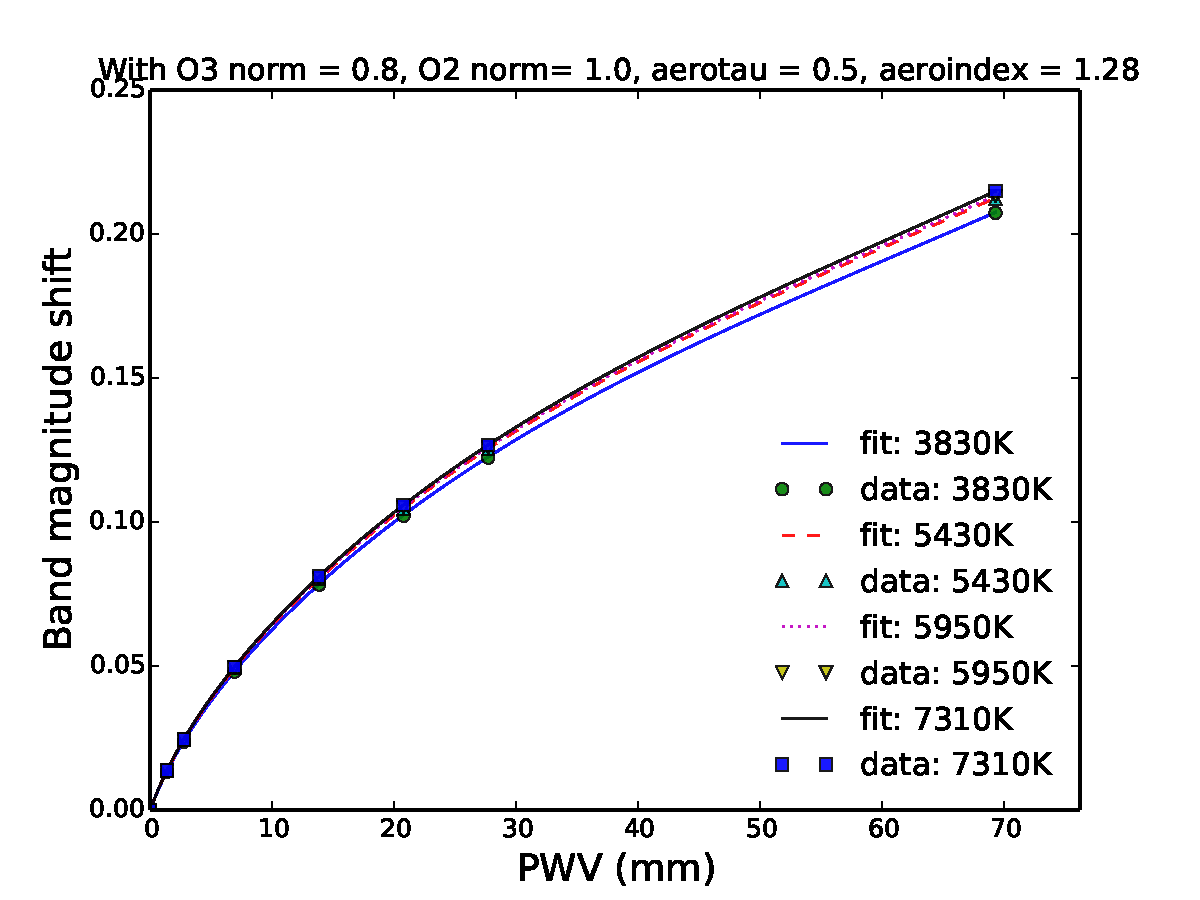
\includegraphics[width=1.\textwidth,trim=5mm 1.5mm 4mm 1.5mm,clip=true,angle=0]{curve_fit_checky_kurucz}
\caption{Check of curve fitting, y band, kurucz stars}
\end{center}
\end{figure}
\FloatBarrier

\clearpage
The residuals of kurucz stars are plotted with PWV=13.86 mm, along the g-r axis. Each color marks a different set of other components (aerosol, O3, O2). The scattering is within 0.001 mag.

\graphicspath{{/home/bruno/users/weh40/Pictures/5figs/}}
\begin{figure}[h!]
\begin{center}
\includegraphics[width=1.\textwidth,trim=1mm 1.5mm 1mm 1.5mm,clip=true,angle=0]{{diserrory1.0}.png}
\caption{fit residuals (in mag.) vs g-r, with PWV=13.86 mm, for y band}
\end{center}
\end{figure}
\FloatBarrier



\clearpage
In summary, the standard deviation and 90 percentile of residuals for both the selected wDs (black) and kurucz (red) stars are plotted against H2O PWV, with wDs std within 0.00013 mag, 90 percentile within0.00025 mag, and those of kurucz within 0.00023 and 0.00035 mag, respectively. This is reasonable, since kurucz stars have a lot of emission/absorption lines. 
\graphicspath{{/home/bruno/users/weh40/Pictures/5figs/}}
\begin{figure}[h!]
\begin{center}
\includegraphics[width=1.\textwidth,trim=1mm 1.5mm 1mm 1.5mm,clip=true,angle=0]{{dise_deviation_sumy}}
\caption{Standard Deviation of fit residuals}
\end{center}
\end{figure}
\FloatBarrier

\clearpage
\subsection{Prediction}


If we know all the other conditions, such as parameters of aerosol, ozone, oxygen, and colors, we can predict the H2O content based on the shift in y band magnitude. The python function we used is scipy.optimize.fsolve.
The pattern of the prediction residuals is similar to that of fit residuals.

\graphicspath{{/home/bruno/users/weh40/Pictures/5figs/}}
\begin{figure}[h!]
\begin{center}
\includegraphics[width=1.\textwidth,trim=1mm 1.5mm 1mm 1.5 mm,clip=true,angle=0]{{cgas_reverse_errory1.0_0}.png}
\caption{PWV prediction residuals vs g-r, with true PWV=13.86 mm, for y band. The black solid line indicate the wDs stars, the red dashed lines indicate the kurucz stars. T}
\end{center}
\end{figure}
\FloatBarrier

 To mimic the realistic situation, we can add noise to the band magnitude. To this end, we will add two uniform distribution noisees of mag 0.002 (S/N = 100 for PWV =  70mm, for which the bands mag. shift $\sim$ 0.21), and 0.01 mag (S/N = 20 for PWV = 70mm).

\paragraph{}
In summary, the prediction residuals in PWV H2O for both wDs and kurucz with and without noises are plotted in the following figure.
\graphicspath{{/home/bruno/users/weh40/Pictures/5figs/}}
\begin{figure}[h!]
\begin{center}
\includegraphics[width=1.\textwidth,trim=1mm 1.5mm 1mm 1.5mm,clip=true,angle=0]{{cgas_deviation_sumy_90}}
\caption{Deviation of prediction residuals, the black color indicates the wDs stars, the red color indicates the kurucz stars. The solid lines are for prediction residuals without noises, dashed lines for noise=0.002 mag, and dotted lines for noise=0.01 mag, and averaged value with 100 stars as well. The standard deviation (std) and 90 percentile (90p) lines are drawn for all cases with and without noises.}
\end{center}
\end{figure}
\FloatBarrier



\paragraph{}
From this figure, it can seen that all kinds of deviation increase with PWV, where the standard deviations of the prediction residuals for both types of stars are around 0.1 mm (PWV = 70 mm), 90 percent residuals around 0.1 - 0.2 mm.

\paragraph{}
With 0.002 mag noise (marked with triangles), there is virtually no distinction between wDs and kurucz stars, and all the prediction residuals are within 0.5 mm for PWV less than 13.86 mm. Their 90 percentiles become worse than 0.5 mm afterwards and reach 1 mm at PWV=70 mm. Averaged with 100 stars (marked with hexgons), the achieved accuracy (estimated based on 90 percentiles) will drop below 0.1 mm for PWV less than 13.86 mm, and become worth than 0.1 mm and reach 0.2 mm for wDs and 0.3 mm for kurucz stars, respectively. 

\paragraph{}
With 0.01 mag noise, the residuals are worse and it is the same for both types of stars. All the 90 percentile residuals are within 2 mm for PWV less than 13.86 mm, and grow worse afterwards and reach 5 mm at PWV=70mm. Averaged with 100 stars (marked with diamonds), the achieved accuracy (estimated with 90 percentiles) will drop below 0.2 mm for PWV less than 13.86 mm, and become worth than 0.2 mm and reach 0.6 mm for wDs and 0.7 mm for kurucz stars, respectively. 

\paragraph{}
(the estimate for what accuracy can be achieved with 100 stars is based on the square root law and considering bias of 90 percentile.)


\clearpage
\begin{thebibliography}{widestlabel}
\bibitem{manual}
The Photon Simulator (Phosim), John R. peterson and the Phosim Group, August 2013
\bibitem{atmoswater}
Ralph FK \& Stephen RS, Nature Vol 358 1992 "Seasonal and interannual variations in atmospheric oxygen and implications for the global carbon cycle"
\end{thebibliography}

\paragraph{}
\textbf{Appendices: } codes for integration (with annotarion)
%\end{document}

\end{document}
